\documentclass[14pt]{extarticle}
\usepackage{fontspec}
\usepackage{polyglossia}
\usepackage{amsmath}
\usepackage{amssymb}
\usepackage{xcolor}
\usepackage{fancyhdr}
\usepackage{graphicx}
\usepackage{listings}
\usepackage[most]{tcolorbox}
% \usepackage{setspace}
\usepackage{pifont}
\usepackage{enumitem}
\usepackage{titlesec}
\usepackage[bottom]{footmisc}
\usepackage{titling}
\usepackage{minted}
\usepackage{etoolbox}
\usepackage{array}
\usepackage{extsizes}
\usepackage{float}
\usepackage{booktabs}
\usepackage{hyperref}
\usepackage[onehalfspacing]{setspace}
\usepackage[a4paper, top=2.7cm, bottom=2.7cm, left=2.5cm, right=2.5cm, headheight=1.5cm, headsep=0.5cm]{geometry}
\usepackage{tikz}

\usetikzlibrary{automata, positioning, arrows.meta, arrows}

\newfontfamily\emoji{Segoe UI Emoji}

\pagestyle{fancy}

\setmainlanguage[numerals=western]{arabic}
\setotherlanguage{english}
% \newfontfamily\arabicfont[Script=Arabic]{Amiri}
\newfontfamily\arabicfont[Script=Arabic]{Calibri}
\newfontfamily\arabicfonttt[Script=Arabic]{Courier New}

\lstset{
  language=[Sharp]C,
  numbers=left,
  stepnumber=1,
  numbersep=8pt,
  frame=single,
  basicstyle=\ttfamily\small,
  keywordstyle=\color{blue},
  stringstyle=\color{red},
  commentstyle=\color{green!50!black}
}

\newif\ifdetailed
\ifdefined\setdetailed
  \setdetailed
\fi

\newif\ifwithsols
\ifdefined\setwithsols
  \setwithsols
\fi

% unified tcolorboxes for articles
\tcbset{colback=white, colframe=black, fonttitle=\bfseries, boxrule=0.8pt}
\newtcolorbox{boxDef}[1][]{colback=blue!5!white,colframe=blue!75!black,
  title={{\emoji📘} تعريف\ifx\\#1\\\else ~#1\fi :}}
\newtcolorbox{boxExercise}[1][]{colback=cyan!5!white,colframe=cyan!70!black,
  title={{\emoji🧩} تمرين\ifx\\#1\\\else ~#1\fi :}}
\newtcolorbox{boxExample}[1][]{colback=yellow!5!white,colframe=orange!90!black,
  title={{\emoji📝} مثال\ifx\\#1\\\else ~#1\fi :}}
\newtcolorbox{boxNote}[1][]{colback=gray!10!white,colframe=black,
  title={{\emoji✨} ملاحظة\ifx\\#1\\\else ~#1\fi :}}
\newtcolorbox{boxAttention}[1][]{colback=magenta!10!white,colframe=magenta!80!black,
  title={{\emoji🔔} تنبيه\ifx\\#1\\\else ~#1\fi :}}
\newtcolorbox{boxWarning}[1][]{colback=red!5!white,colframe=red!75!black,
  title={{\emoji⚡} ملاحظة هامة\ifx\\#1\\\else ~#1\fi :}}
\newtcolorbox{boxSolution}[1][]{colback=green!5!white,colframe=green!60!black,
  title={{\emoji✅} حل\ifx\\#1\\\else ~#1\fi :}}
\newtcolorbox{boxSymbol}[1][]{colback=purple!5!white,colframe=purple!70!black,
  title={{\emoji🔣} رمز\ifx\\#1\\\else ~#1\fi :}}
\newtcolorbox{boxHint}[1][]{colback=teal!5!white,colframe=teal!60!black,
  title={{\emoji💡} تلميح\ifx\\#1\\\else ~#1\fi :}}


\tcbset{simplecode/.style={ colback=gray!5, colframe=black!50, boxrule=0.4pt, arc=2pt, left=4pt,right=4pt,top=4pt,bottom=4pt}}
\newenvironment{boxCode}{\begin{tcolorbox}[simplecode]}{\end{tcolorbox}}

\newcolumntype{C}[1]{>{\centering\arraybackslash}p{#1}}

% redefine spaces after titles
\makeatletter
\renewcommand{\@maketitle}{%
  \begin{center}
    {\huge \bfseries \@title \par}%
    \vskip 0.2em % space between title and author
    {\large \@author \par}%
    % \vskip 0.2em % space between author and date
    % {\normalsize \@date \par}%
  \end{center}
}
\makeatother

\fancyhf{} % clear default
\fancypagestyle{plain}{
  \fancyhf{}
  \fancyhead[L]{مدرسة التسامح الشاملة}
  % \fancyhead[L]{
\includegraphics[height=1cm]{../../../images/logoTasamoh.png}}
  \fancyhead[R]{الأستاذ محمود اغبارية}
  \fancyfoot[C]{\thepage}
}

\fancyhead[L]{مدرسة التسامح الشاملة}
\fancyhead[R]{الأستاذ محمود اغبارية}
\fancyfoot[C]{\thepage}
% \date{\today}

\setcounter{tocdepth}{3} % only section subsection and subsubsection in TOC

\newcommand{\importpdfpage}[2]{%
    \thispagestyle{empty}
    \newgeometry{left=0cm,right=0cm,top=0cm,bottom=0cm}
    \includegraphics[page=#2,width=0.95\paperwidth,height=0.95\paperheight,keepaspectratio]{#1}
    \restoregeometry
}

\newcommand{\insertFullImg}[1]{%
    \noindent
    \makebox[\textwidth][c]{
        \includegraphics[width=0.9\paperwidth,keepaspectratio]{#1}%
    }%
}%

% ----------------------


% \begin{document}

% \maketitle

% % \clearpage  % start TOC on a new page
% % \renewcommand{\contentsname}{جدول المحتويات}
% % \tableofcontents
% % \clearpage

% \part*{part 1} % the * prevents numbering
% \section*{مقدمة}
% \subsection*{مثال رياضي}
% \subsubsection*{مثال فرعي}
% \paragraph*{ paragraph 1}
% \subparagraph*{sub paragraph 1}

% \ifdetailed
% \begin{english}
% \begin{minted}{csharp}
% // C# Example
% \end{minted}
% \end{english}
% \fi

% OLD WAY
% \ifdetailed
% \begin{english}
% \begin{lstlisting}
% // C# Example
% \end{lstlisting}
% \end{english}
% \fi

% % 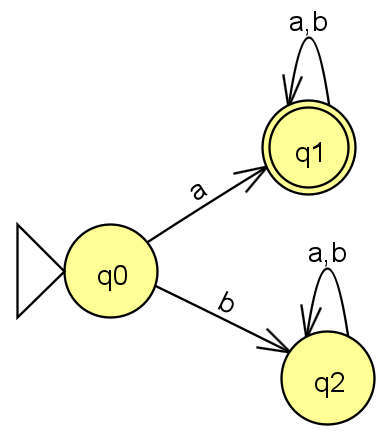
\includegraphics[width=0.2\textwidth]{../../../images/DFAs/ex1_q1.png}



% \vspace{3cm}
% \begin{flushleft}
% أرجو لكم وقتًا ممتعًا.

% الأستاذ محمود اغبارية.
% \end{flushleft}


% \end{document}


\title{المتغيرات والعمليات الحسابية}

\begin{document}
\maketitle

\section{المتغيرات}

تعريف المتغيرات يكون بواسطة الأمر التالي:

\begin{boxExample}
\begin{english}
\begin{minted}{csharp}
var_type var_name = var_value;
\end{minted}
\end{english}
\end{boxExample}

\begin{itemize}
\item \textenglish{var\_type} هو نوع المتغير
\item \textenglish{var\_name} هو اسم المتغير
\item \textenglish{var\_value} هي قيمة المتغير.
\end{itemize}

\subsection{أنواع المتغيرات في لغة \textenglish{C\#}}
أنواع المتغيرات التي سنستخدمها في \textenglish{C\#} هي:

\begin{center}
\begin{tabular}{|c|c|c|}
\hline
النوع & مثال & الوصف \\
\hline
\textenglish{int} & \textenglish{int x = 5;} & عدد صحيح (\textenglish{Integer}) \\
\hline
\textenglish{double} & \textenglish{double y = 3.14;} & عدد عشري (\textenglish{Floating-point}) \\
\hline
\textenglish{string} & \textenglish{string name = "Ali";} & سلسلة نصية (\textenglish{Text}) \\
\hline
\textenglish{char} & \textenglish{char grade = 'A';} & حرف واحد (\textenglish{Character}) \\
\hline
\textenglish{bool} & \textenglish{bool flag = true;} & قيمة منطقية (\textenglish{True/False}) \\
\hline
\end{tabular}
\end{center}

\begin{boxExample}
\begin{english}
\begin{minted}{csharp}
int x = 5;
double y = 3.14;
string name = "Ali";
char grade = 'A';
bool flag = true;

Console.Write("x = "); // Prints the expression "x ="
Console.WriteLine(x); // Prints the value of x with a new line
Console.Write("y = "); // Prints the expression "y ="
Console.WriteLine(y); // Prints the value of y with a new line
Console.Write("name = "); // Prints the expression "name ="
Console.WriteLine(name); // Prints the value of name with a new line
Console.Write("grade = "); // Prints the expression "grade ="
Console.WriteLine(grade); // Prints the value of grade with a new line
Console.Write("flag = "); // Prints the expression "flag ="
Console.WriteLine(flag); // Prints the value of flag with a new line
\end{minted}
\end{english}
\end{boxExample}

\textbf{قوانين وملاحظات مهمة لتسمية المتغيرات:}
\begin{itemize}
\item اسم المتغير مكون من: أحرف، أرقام، شَرطة سفلية (\textenglish{\_}) - يمنع استخدام رموز أخرى.
\item اسم المتغير يجب أن يبدأ بحرف (يمكن أن يبدأ أيضًا بشرطة سفلية، لكن هذا غير مفضل إلا في حالات خاصة)
\item أسماء المتغيرات حساسة لحالة الأحرف (كبيرة أو صغيرة)
\item يجب اختيار اسم معبّر للمتغير، مثلا: \textenglish{grade}, \textenglish{age}, \textenglish{name}, \textenglish{id}...
\item اسم المتغير ونوعه لا يمكن تغييرهما، أمّا القيمة فيمكن تغييرها لاحقًا خلال البرنامج
\item إذا كان اسم المتغير مكوّنًا من أكثر من كلمة، فالمتّبع أنّ أول حرف من كل كلمة ابتداء من الكلمة الثانية يبدأ بحرف كبير.
\end{itemize}

\begin{center}
\begin{tabular}{|c|c|c|}
\hline
اسم قانوني & اسم غير قانوني & اسم قانوني لكن غير مفضل \\
\hline
\textenglish{name} & \textenglish{name-1} & \textenglish{Name} \\
\hline
\textenglish{grade1} & \textenglish{grade\#1} & \textenglish{gg} \\
\hline
\textenglish{firstName} & \textenglish{first name} & \textenglish{firstname} \\
\hline
\textenglish{isEven} & \textenglish{isEven?} & \textenglish{isNotEven} \\
\hline
\end{tabular}
\end{center}

\begin{itemize}
\item يمكن تأخير إعطاء القيمة للمتغير:
\end{itemize}

\begin{boxExample}
\begin{english}
\begin{minted}{csharp}
var_type var_name;
var_name = var_value;
\end{minted}
\end{english}
\end{boxExample}

\begin{center}
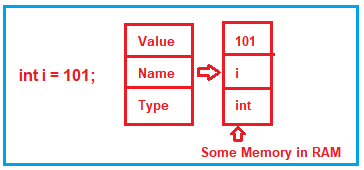
\includegraphics[width=0.5\textwidth]{../../../images/variable_in_memory.png}
\end{center}

\begin{boxExample}
\begin{english}
\begin{minted}{csharp}
double pi; // Defining a variable of type double, but it cannot be used before assigning a value
pi = 3.14; // Assigning a value to the variable pi, now it can be used
Console.WriteLine("pi = " + pi);
pi = 3.14159265359; // The value of the variable can be changed at any time
Console.WriteLine("pi = " + pi);
\end{minted}
\end{english}
\end{boxExample}

\begin{itemize}
\item إعطاء قيمة للمتغير هو عملية نسخ للقيمة
\end{itemize}

\begin{boxExample}
\begin{english}
\begin{minted}{csharp}
int n1 = 10;
int n2 = n1;
Console.WriteLine(n2);
n1 = 20;
Console.WriteLine(n2);
n2 = n2 + 3;
Console.WriteLine(n2);
Console.WriteLine(n1);
\end{minted}
\end{english}
\end{boxExample}

\subsection{القيم القصوى والدنيا لأنواع المتغيرات}

\begin{itemize}
\item القيم التي يمكن أن يأخذها متغير في البرمجة هي قيم محدودة، وليست لا نهائية.
\item لكل نوع من أنواع المتغيرات يمكننا فحص القيمة القصوى والقيمة الدنيا له باستخدام الخصائص \textenglish{MinValue} و \textenglish{MaxValue}
\end{itemize}

\begin{boxExample}
\begin{english}
\begin{minted}{csharp}
Console.WriteLine(int.MaxValue);
Console.WriteLine(int.MinValue);
Console.WriteLine(double.MaxValue);
Console.WriteLine(double.MinValue);
\end{minted}
\end{english}
\end{boxExample}

\subsection{العمليات الحسابية على المتغيرات}

\begin{itemize}
\item يمكننا استعمال المتغيرات مع عمليات حسابية.
\item التعابير الحسابية تراعي ترتيب العمليات الحسابية (الضرب والقسمة قبل الجمع والطرح)
\end{itemize}

\begin{boxExample}
\begin{english}
\begin{minted}{csharp}
int a = 10;
int b = 2;
Console.WriteLine(a + b); // Addition
Console.WriteLine(a - b); // Subtraction
Console.WriteLine(a * b); // Multiplication
Console.WriteLine(a / b); // Division
Console.WriteLine(a % b); // Modulus (Remainder)
Console.WriteLine(a + 2 * b); // Order of operations is considered: multiplication before addition.
Console.WriteLine((a + b) * (a - b)); // Using parentheses to change the order of operations
\end{minted}
\end{english}
\end{boxExample}

\subsection{قراءة من المستخدم}

\begin{itemize}
\item لقراءة معطيات من المستخدم نستعمل الأمر التالي:
\textenglish{Console.ReadLine();}
\item هذا الأمر \textbf{دائمًا} يرجع قيمة من نوع \textenglish{String}
\item \textbf{يجب} طباعة رسالة للمستخدم قبل قراءة المعطى تشرح للمستخدم ماذا عليه أن يُدخل
\item لكي نستقبل رقمًا من المستخدم نقوم بالتالي:
\end{itemize}

\begin{boxExample}
\begin{english}
\begin{minted}{csharp}
Console.WriteLine("Please enter your age as integer: ");
String sAge = Console.ReadLine();
int age = int.Parse(sAge);
Console.WriteLine("your arge is: " + age);
\end{minted}
\end{english}
\end{boxExample}

\begin{itemize}
\item بنفس الطريقة يمكننا استخدام \textenglish{double.Parse(s)}.
\end{itemize}

\subsection{تحويل بين \textenglish{int} و \textenglish{double}}

كل عدد صحيح هو عدد عشري بشكل طبيعي، فالتحويل من \textenglish{int} إلى \textenglish{double} مفهوم وواضح.

انتبه أنّ \textenglish{double} يمكنه استقبال عدد صحيح (لأنّ العدد الصحيح هو عدد عشري)

\begin{boxExample}
\begin{english}
\begin{minted}{csharp}
double numDouble = 5;
Console.WriteLine(numDouble);
int numInt = 12;
numDouble = numInt;
Console.WriteLine(numDouble);
\end{minted}
\end{english}
\end{boxExample}

إذا أردنا التحويل بالاتجاه المعاكس (أي من \textenglish{double} إلى \textenglish{int})، فهذا الأمر سيؤدي إلى مشكلة، لأنّه ليس كل عدد عشري هو عدد صحيح.

في هذه الحالة لا بدّ من أن نخبر الحاسوب أنّنا نريد تحويل العدد العشري إلى عدد صحيح عن طريق إضافة \textenglish{(int)} قبل العدد العشري، وعندها سيحوّل الحاسوب العددَ العشري إلى عدد صحيح عن طريق حذف الجزء الكسري منه

\begin{boxExample}
\begin{english}
\begin{minted}{csharp}
double numDouble2 = 5.24;
int numInt2 = (int) numDouble2;
Console.WriteLine(numInt2); // Prints 5 only, because the fractional part was removed
\end{minted}
\end{english}
\end{boxExample}

\textbf{انتبه} التحويل من عدد صحيح إلى عشري هو تحويل تلقائي، لأننا لن نخسر معه معلومات.
أمّا التحويل من عدد عشري إلى عدد صحيح فيجب علينا أن نفعل ذلك بشكل واضح ومفصل عن طريق إضافة \textenglish{(int)} لأنّنا سنخسر بعض المعلومات (الجزء الكسري من العدد سيضيع)

\subsection{عمليتا القسمة والباقي}

\subsubsection*{عملية القسمة}

عند قسمة عددين صحيحين، فالنتيجة دائمًُا تكون عددًا صحيحًا. أي إذا كانت الإجابة تحتوي على كسور فإنّها تُحذف ويبقى العدد الصحيح فقط.

\begin{boxExample}
\begin{english}
\begin{minted}{csharp}
int i1 = 8;
int j1 = 3;
Console.WriteLine(i1 / j1);
\end{minted}
\end{english}
\end{boxExample}

بالمقابل، إذا قسّمنا عددين عشريّين (من نوع \textenglish{double}) فإنّ النتيجة ستكون عشرية أيضًا:

\begin{boxExample}
\begin{english}
\begin{minted}{csharp}
double d1 = 8;
double d2 = 3;
Console.WriteLine(d1 / d2);
\end{minted}
\end{english}
\end{boxExample}

وأيضًا إذا قسّمنا عددين أحدهما عشري والآخر صحيح، فالنتيجة عشرية (بغض النظر أيهما البسط أو المقام):

\begin{boxExample}
\begin{english}
\begin{minted}{csharp}
int i2 = 8;
double d3 = 3;
Console.WriteLine(i2 / d3);
Console.WriteLine(d3 / i2);
\end{minted}
\end{english}
\end{boxExample}

إذا أردنا تقسيم عددين صحيحين والحصول على نتيجة عشرية، فلا بد من تحويل أحد العددين إلى عدد عشري قبل القسمة عن طريق إضافة \textenglish{(double)} قبل العدد:

\begin{boxExample}
\begin{english}
\begin{minted}{csharp}
int i2 = 8;
int j2 = 3;
Console.WriteLine(i2 / j2); // The result will be 2 only, because we are dividing two integers
Console.WriteLine(((double)i2) / j2); // The result will be 2.66666666666667, because we converted i2 to a decimal number
Console.WriteLine(i2 / ((double) j2)); // The result will be 2.66666666666667, because we converted j2 to a decimal number
\end{minted}
\end{english}
\end{boxExample}

بالمقابل، إذا أردنا تقسيم عددين عشريين والحصول على نتيجة بصورة عدد صحيح (أي لا نريد الجزء الكسري) فيمكننا تحويل النتيجة إلى عدد صحيح عن طريق إضافة \textenglish{(int)} قبل التعبير

\begin{boxExample}
\begin{english}
\begin{minted}{csharp}
double d3 = 8.0;
double d4 = 3.0;
int i3 = (int)(d3 / d4);
Console.WriteLine(i3);
\end{minted}
\end{english}
\end{boxExample}

\textbf{للتلخيص}

\begin{itemize}
\item قسمة عددين لهما نفس النوع تكون من نفس نوعهما.
\item إذا كان أحد الأعداد في القسمة عشريًّا (\textenglish{double}) فالنتيجة دائمًا عشرية
\item إذا أردنا تحويل تعبير إلى عدد صحيح فإنّنا نضيف قبله \textenglish{(int)}.
\item إذا أردنا تحويل تعبير إلى عدد عشري فإنّنا نضيف قبله \textenglish{(double)}.
\end{itemize}

\textbf{تمرين}:
\begin{enumerate}
\item استقبل من المستخدم 3 علامات، ثم اطبع له معدّله
\item استقبل من المستخدم 3 علامات، ولكل علامة استقبل عدد الوحدات، ثم اطبع له المعدّل.
\end{enumerate}

\subsection{عملية الباقي \textenglish{\%}}

الباقي بين عددين معرّف على أنّه الفرق بين العدد المقسوم وأكبر عدد أصغر منه يقسم عليه العدد مقسوم عليه.

مثلًا: باقي قسمة 20 على 6 هو 2، لأن:
\begin{itemize}
\item العدد المقسوم هو 20
\item العدد المقسوم عليه هو 6.
\item أكبر عدد أصغر من 20 يقسم عليه 6 هو 18.
\item الفرق بين 18 و 20 هو 2
\item إذن اقي قسمة 20 على 6 هو 2.
\end{itemize}

يمكننا إجراء عملية الباقي بين متغيرات من نوع \textenglish{int} و \textenglish{double} في لغة \textenglish{C\#} عن طريق استخدام العملية \textenglish{\%}

\begin{boxExample}
\begin{english}
\begin{minted}{csharp}
Console.WriteLine("7 % 4 = " + (7 % 4)); // Prints 3, which is the remainder of 7 divided by 4
Console.WriteLine("12 % 3 = " + (12 % 3)); // Prints 0, because 12 is divisible by 3 without a remainder
Console.WriteLine("100 % 6 = " + (100 % 6)); // Prints 4, which is the remainder of 100 divided by 6
Console.WriteLine("3 % 10 = " + (3 % 10)); // Prints 3, because 3 is smaller than 10, so the remainder is 3 itself

int n1 = 20;
int n2 = 6;
Console.WriteLine($"n1 % n2 = {n1} % {n2} = " + (n1 % n2)); // Prints 2, which is the remainder of 20 divided by 6
\end{minted}
\end{english}
\end{boxExample}

من أهم استخدامات عملية الباقي هو تجزئة العدد إلى خاناته المكون منها.

عندما نحسب باقي عدد ما على 10، فإنّنا سنحصل على خانة الآحاد في العدد.

ثم يمكننا قسمة العدد على 10، ثم أخذ باقي النتيجة على 10 فنحصل على خانة العشرات... وهكذا

\begin{boxExample}
\begin{english}
\begin{minted}{csharp}
int n = 847;
int originalNumber = n; // We keep a copy of n to use it later in printing
Console.WriteLine(n);

int units = n % 10; // Units digit
n = n / 10; // Remove units digit
Console.WriteLine("n after deleting units digit = " + n);

int tens = n % 10; // Tens digit
n = n / 10; // Remove tens digit
Console.WriteLine("n after deleting tens digit = " + n);

int hundreds = n % 10; // Hundreds digit
n = n / 10; // Remove hundreds digit (now n should be 0)
Console.WriteLine("n after deleting hundreds digit = " + n);

Console.WriteLine($"Original number = {originalNumber}, Hundreds = {hundreds}, Tens = {tens}, Units = {units}");
\end{minted}
\end{english}
\end{boxExample}

\clearpage

\subsection{مكتبة العمليات الرياضية (\textenglish{Math})}

لغة \textenglish{C\#} توفّر مكتبة جاهزة اسمها \textenglish{Math} تحتوي على مجموعة من الدوالّ الرياضية المفيدة للتعامل مع الأرقام، ومنها:

\begin{center}
\begin{tabular}{|c|c|c|}
\hline
العملية & الوصف & مثال \\
\hline
\textenglish{Math.Sqrt(x)} & حساب الجذر التربيعي للعدد $\mathbf{x}$ & \textenglish{Math.Sqrt(16)} \\
\hline
\textenglish{Math.Max(x, y)} & إرجاع أكبر قيمة من بين $\mathbf{x}$ و $\mathbf{y}$ & \textenglish{Math.Max(10, 5)} \\
\hline
\textenglish{Math.Min(x, y)} & إرجاع أصغر قيمة من بين $\mathbf{x}$ و $\mathbf{y}$ & \textenglish{Math.Min(10, 5)} \\
\hline
\textenglish{Math.Pow(x, y)} & حساب $\mathbf{x}$ مرفوعًا للقوة $\mathbf{y}$ ($x^y$) & \textenglish{Math.Pow(2, 3)} \\
\hline
\textenglish{Math.Abs(x)} & حساب القيمة المطلقة للعدد $\mathbf{x}$ & \textenglish{Math.Abs(-7)} \\
\hline
\textenglish{Math.Round(x)} & تقريب العدد $\mathbf{x}$ إلى أقرب عدد صحيح & \textenglish{Math.Round(4.7)} \\
\hline
\end{tabular}
\end{center}

\textbf{ملاحظة هامة:} معظم دوال \textenglish{Math} (مثل \textenglish{Sqrt} و \textenglish{Pow} و \textenglish{Round}) تتعامل مع نوع \textenglish{double} وتُرجع قيمة من نوع \textenglish{double}.

\begin{boxExample}
\begin{english}
\begin{minted}{csharp}
// Examples of using Math library functions

double x = 16.0;
double y = 4.7;
int a = 10;
int b = 25;

// 1. Square Root (Sqrt)
double sqrtX = Math.Sqrt(x);
Console.WriteLine($"The square root of {x} is: {sqrtX}");

// 2. Maximum Value (Max)
int maxAB = Math.Max(a, b);
Console.WriteLine($"The maximum of {a} and {b} is: {maxAB}");

// 3. Minimum Value (Min)
int minAB = Math.Min(a, b);
Console.WriteLine($"The minimum of {a} and {b} is: {minAB}");

// 4. Power (Pow)
double powResult = Math.Pow(2, 5); // 2^5
Console.WriteLine($"2 to the power of 5 is: {powResult}");

// 5. Absolute Value (Abs)
int absResult = Math.Abs(-15);
Console.WriteLine($"The absolute value of -15 is: {absResult}");

// 6. Rounding (Round)
double roundY = Math.Round(y);
double roundY2 = Math.Round(4.3);
Console.WriteLine($"Rounding {y} gives: {roundY}");
Console.WriteLine($"Rounding 4.3 gives: {roundY2}");
\end{minted}
\end{english}
\end{boxExample}

\end{document}